\documentclass[12pt,a4paper,oneside]{book} 
%scrbook book report

\usepackage{multirow}
\usepackage{graphicx}
\usepackage[table]{xcolor}
\usepackage{float}
%\usepackage{color}
%\usepackage{subfigure}
\usepackage{seecs}
%\usepackage{color}
%\usepackage{colortbl}
%\usepackage{soul}
%\usepackage{listings}
%\lstloadlanguages{Java,XML}
%\lstset{frame=lines}
%\usepackage{astron}
%\usepackage{xspace}
%\usepackage[leqno]{amsmath}
%\usepackage{hyperref}
%\usepackage{sfmath}
%\usepackage{setspace}
\usepackage{cite}
\definecolor{lightgray}{gray}{0.9}


%\usepackage{amsmath,amssymb,amsthm,paralist}
%% Include other packages you wish to use except setspace.
%% That package is loaded automatically.
%% IMPORTANT: Load only those packages you know you will use.
%% Some packages can cause conflicts resulting in improper formatting.
%\usepackage{graphicx}
%\usepackage{subfig}
%\usepackage{latexsym}
%\usepackage{url}
%%\usepackage{soul}  % package for strikeout \st{}
%\usepackage{algorithm}
%\usepackage{algorithmic}
\usepackage{cite}
\renewcommand{\baselinestretch}{1.5}


\title{Automating Exchange of Educational Certificates Using DRESS}
%\subtitle{An optional sub-title, usually not used at NUST}

\author{Umair Anwar}
\regno{2011-NUST-MS PhD-IT-049}
\degree{\MSIT} 
% Argument pptions for \degree{_____}:
% \BSIT for Bachelor of Science in Information Technology (BS IT)
% \BSCS for Bachelor of Science in Computer Science (BS CS)
% \BICSE for Bachelor of Engineering in Information and Communication Systems (BE ICS)
% \BEE for Bachelor of Engineering in Electronics (BE Electronics)
% \MSIT for Masters of Science in Information Technology (MS IT)
% \MSCSE for Masters in Communication Systems Engineering (MS CSE)
% \MSCCS for Masters in Computer and Communication Security (MS CCS)
% \MSEE for Masters of Science in Electrical Engineering (MS EE)

\adviser{Dr. Sharifullah Khan}
\adviserAffiliation{Department of Computing}

\date{June 2015}

%\setcounter{tocdepth}{2}
 %\setstretch{1.1}
 %\linespread{1.1}

\begin{document}
\maketitle

\evaluationcommitteeapproval{Dr. Hamid Mukhtar}{Dr. Sarah Shafiq Khan}{Mr. Mujtaba Haider}

\chapter*{Abstract}

 Bologona process aimed to ease the mobility of students across Europe. Previously, some efforts were made in related domains but these were not focused on mobility of the students between institutes. Hence, efforts were put developing standards and proposing suitable architectures that fit all across Europe under the umbrella of Bologna process. Inspired by this, the mobility project tried to gather and reuse all the work previously done in related areas. Mobility reused the vocabularies, ideas and focused on the mobility of students. However, it created an opportunity for a semi-automated mapping tool for mapping proposed standard to the heterogeneous schema of different institutes. It lacks enough vocabulary to cover exchange of information for some educational certificates in Pakistan.
 
 We suggest a prototype infrastructure that provides more control and improves this exchange of information between partaking institutes by covering more detailed vocabulary. The term infrastructure includes both the architecture and our proposed standard (DRESS). 
 
 We avail the opportunity that The Mobility Project provided and suggest a mapping tool that semi-automatically create mappings between our standard and the heterogeneous data-sets of different partaking institutes. 

%---------------------------------------------------------------------
\certificateoforiginality
%---------------------------------------------------------------------
\chapter*{Acknowledgment}
All gratefulness and wonderfulness to {\bfseries ALLAH} and with His blessings, i am in good health and he gave me the ability to complete this work. I pray for more of Allah's blessings. It would not be possible without the efforts that were made by my {\bfseries parents} for supporting me during this duration and throughout my life. 

I am truly thankful to my supervisor {\bfseries Dr. Sharifullah Khan} for his guidance and who had been a great coach. I want to express my gratitude towards him for believing in me and facilitating me for the completion of this work. I appreciate {\bfseries Dr. Hamid Mukhtar}, {\bfseries Dr. Sarah Shafiq Khan} and {\bfseries Mr. Mujtaba Haider} for suggesting me and for their support. 

I am thankful to all my colleagues, co-workers and contributors who were supportive in completing this research.

\begin{flushright} \textbf{Umair Anwar} \end{flushright}
%---------------------------------------------------------------------

\tableofcontents
%
%\printnomenclature{2.5cm}
%\nomenclature{DCF}{Distributed Coordination Function}
%
%
\chapter*{List of Abbreviations}

\begin{table}[h]
   % increase table row spacing, adjust to taste
    \renewcommand{\arraystretch}{1.3}
    \label{table:table1}
     \begin{tabular}{ll}
        \hline\hline
        % inserting double-line
            {\bfseries Abbreviations} & {\bfseries Descriptions} \\
            \hline                                      % inserts single-line
            DRES & Document Record Exchange Standard  \\
            DRESS & Document Record Exchange Standard Secured  \\
            SCHAC & Schema for Academia  \\
            LDAP & Lightweight Directory Access Protocol \\
            FVUSPEC & Finnish Virtual University Specifications  \\
            MLO & Meta-data for Learning Opportunities  \\
            WSDL & Web Service Description Language  \\
            EHEA & European Higher Education Area  \\
            ECTS & European Credit Transfer and Accumulation System  \\
            EA & Exchange Agreement  \\
            NQF & National Qualifications Framework  \\
            EQF & European Qualifications Framework  \\
            \hline                          % inserts single-line
    \end{tabular}
\end{table}

\listoffigures
\listoftables
% \lstlistoflistings

\resetpagenumbering
%---------------------------------------------------------------------

\chapter{Introduction}\label{ch-intro}
%-----------------------------------------------

With time passing, the exchange of official and legal documents digitally is getting more and more importance. In near future, it will be inevitable to transform our systems to facilitate this change. Same is the case with the exchange of educational certificates between different partaking institutes and authorities. Its importance can be imagined by the number of students and institutes involved. 

In 1999, it was decided in Bologna declaration to create European Higher Education Area which facilitate to standardize the exchange of information across Europe. Alone in Europe, more than four thousands partaking institutes with more than two million students were involved in this process in academic year 2009-2010. 

Enter Universities and students statistics from Pakistan.

It is a well established fact that more and more systems are digitized every year. The educational institutes are also making their record digital and this trend is increasing. For example, more and more universities are implementing electronic student information systems to keep student courses and credit record. However, the documents often called degrees/certificates issued by these autonomous bodies are still exchanged in paper form.  

This manual approach of exchanging physical documents and re-enter the data again manually in digital or physical for by people is error prone and exhaustive. As a result the local data-sets of these autonomous bodies has different record for the same individual. 

This creates an opportunity for a common data-exchange standard which bring a common ground for the exchange of information. To resolve the issues facing in manual exchange of documents, the institutional systems must talk to each other using a common standard. This would make the entire process more dependable and less error prone.

This research digs into the currently adopted solutions, standards and the new research in the area of student mobility and exchange of official documents related to students. It suggests a prototype infrastructure including data format and the architecture to exchange degree records digitally. 

Each institutional system is an autonomous body maintaining its data separately. The schema of the data is different in different institutes. For our proposed architecture and standard to work, each institute must  implement web-services based on DRESS for the exchange of documents. This approach is very time consuming, inefficient, and error prone. This provides us another  opportunity to suggest a tool that maps these different types of databases schema from different institutes to DRESS. 

To handle the different levels of heterogeneity, we came up with a mapping tool which semi-automatically maps institutes data-sets to our proposed standard and creates web-services to access their data.

The rest of the chapter is organized as follows. In Section \ref{s-problem_statement}, the problem statement is stated. In Section \ref{s-contributions}, thesis contributions are stated. In Section \ref{s-thesis-organization}, we conclude the chapter with an outline for the rest of the thesis.

The remaining chapter is sorted out as this; In Section 1.1, we explain the problem Statement. In Section 1.2, we discuss what this research has contributed. In Section 1.3, we explain how this research is organized into chapters.

\section{Problem Statement}\label{s-problem_statement}

""

\section{Contributions}\label{s-contributions}

Our research work contributes in .................. areas.

All contributions of ................. are summarizing as follows:

\subsection{Motivation}

\begin{itemize}
\item

\item
Finding 2.
\end{itemize}

\subsection{Goals}

\begin{itemize}
\item
Implementation of a mapping tool to ease mapping of heterogeneous schema with our proposed standard DRESS.
\item
Suggesting a suitable prototype architecture for the exchange of educational certificates such that 
every data owning entity is the owner of its own data to build trust
have built-in control for authenticity
\item
Propose a generic and extendable standard for the exchange of educational certificates with well defined vocabulary.
\end{itemize}

\subsection{Challenges}

\begin{itemize}
\item
Finding 1.
\item
Finding 2.
\end{itemize}

\section{Thesis Organization}\label{s-thesis-organization}

The rest of the thesis is organized as follows: \\

Chapter 2 discusses the state of the art related to the current research, and reviews the relevant literature aimed at finding

In Chapter 3, the .................... are discussed and then proposed methodology is presented. \\

In Chapter 4, the results are given along with detailed discussions. \\

In Chapter 5, the conclusion and future work is presented.

\chapter{Literature Review}\label{ch-work}

There already exists a few standards and practices identified with exchanging degree or courses record. It is important to go through these, before proceeding onward to the new standard and the architecture we are proposing. We will review what these standards cover and what we can reuse.

\section{Bologna Process}

It intends to make European educational framework of standards engaging different countries in Europe to compare, contrast and make compatible their educational systems. \cite{bologna process}

To improve the mutual recognition of degrees and programs, education ministers from 29 countries signed bologna declaration in 1999. Other partaking countries joined the program later. \cite{improvement bologna process} Bologna process is quite often named as European Higher Education Area (EHEA). EHEA focuses on transferal and convergence adaption by 46 countries. This process benefits Europeans and it has its significance for other educational institutes and communities. a) The leading role of European institutes, b) the lessons that are learned in the implementation of the framework of standards, and c) the practices adopted guide the educational communities around the world. 2010 was marked as the deadline across Europe for implementing the agreed specifications. \cite{European Higher Education Area }

To meet the 2010 deadline, Spain started to implement the convergence of undergraduate engineering degrees that conformed EHEA in 2008. This standardization provided some opportunities for mobility and unified measurements. \cite{European Higher Education Area }




\section{Qualifications Exchange Standards}

    \subsection{European Qualifications Framework}
    EQF is an agreed reference framework that helps participating countries to compare national qualifications and make them more clear, readable and understandable across Europe. The point is to advance mobility of workers and learners. This was settled upon by European universities in 2008 to relate their national qualifications to EQF. The new qualifications from 2012 carry a reference to suitable EQF level.

    EQF comprises of eight reference levels, each showing what a learner knows and has the capacity to understand it. National qualifications of the partaking countries identify and relate with these eight levels raging from basic (level 1) to advanced (level 8) as shown in figure ~\ref{fig:EQF}. This simplifies qualification comparison in partaking countries supporting mobility of learners and empowering them to not repeat what they have already learned.

\begin{figure}[!hbp]
  \centering
  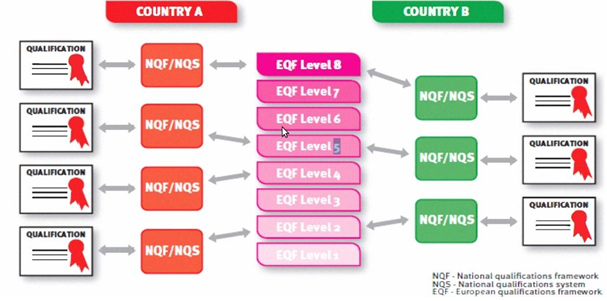
\includegraphics[width=14cm]{eqf.png}
  \caption{EQFs against NQFs \cite{MAPQFTOOL}}
  \label{fig:EQF}
\end{figure}

    EQF concentrates on learning results as opposed to concentrating on learning inputs. It covers all types of education including professional, vocational and school education. It tries to validate formal and in addition informal education.

    \subsection{Europass}
    Collection of five documents which intend to ease mobility when seeking employment across Europe. These include the Curriculum Vitae, the Language Passport, the Mobility, the Diploma Supplement, and the Certificate Supplement. One can fill himself the Curriculum Vitae, and the Language Passport but the rest of the documents are issued by the related authorities. It follows a standard template format system, a layout. Same format helps to achieve neutrality and transparency while presenting one's skills.

    The motto as mentioned on the Europass website's homepage is as follows;
    "Five documents to make your skills and qualifications clearly and easily understood in Europe"

    Europass has defined XML schemas for CV and Language Passport. The documents can be exported in XML format when created on Europass. These exported XML documents can be imported to Europass and converted to HTML, PDF, Microsoft Word or ODT templates.

    Europass specifies JSON schema according to Internet Engineering Task Force's JSON specifications draft. The europass JSON vocabulary is close and similar to europass XML schema. The JSON objects for europass documents (CV and Language Passport) can be validated using Europass JSON validator.

    All these documents have some common XML schema attributes which describe document type, printed preferences.

    Europass does not explain details related to degrees or educational certificates in XML certificate.

        \subsubsection{Europass Curriculum Vitae}
        Europass Curriculum Vitae (ECV) is a template which one can create online and it can be exported in xml format. The ECV XML schema contains vocabularies related to document type, printing preferences, personal details, contact details, skills, and educational degrees and institutes. The XML vocabulary related to degree details is very little only to cover the scope of a CV.

        \subsubsection{Europass Language Passport}
        Europass Language Passport (ELP) is a template. One can create it online and export it in europass xml format. It contains XML vocabulary related to language skills and the scale of six values to score proficiency.

    \subsection{Schema for Academia}
    The need for the inter-exchange of information between institutes across Europe has highlighted the importance of common attributes for this exchange to take place. Schema for Academia (SCHAC) is the result of the attribute coordination between different institutes. It plans to define and advance common attributes in the field of higher education to encourage data-exchange between institutions. It does not plan to supplement different the national schemas, rather it suggests a coordinated framework on top of the different national schemas.
    
    Schema for Academia (SCHAC) describes vocabulary related degrees and courses. The schema is not technology dependent and written for LDAP (Lightweight Directory Access Protocol). It aims at promoting a common framework to inter-exchange data between educational institutes. It defines attributes that describe individuals and their LDAP profile.
    
	It is a collection of schemas which can be classified into following categories;
\begin{itemize}
\item
Personal Characteristics
\item
Location Information
\item
Student Information
\item
Employee Information
\item
Linkage Identifiers
\item
Administration Information
\item
Confidentiality (Visibility)
\item
Authorization, Entitlements
\item
Group-related Attributes
\end{itemize}

	SCHAC has a clearly defined meta-information for defining an attribute. To discuss the ideas  used by SCHAC, let us look in detail the schacGender attribute as an example shown in Table \ref{tab:schacGender}. It uses ISO-standards where-ever possible. In schacGender attribute, it is using values from ISO-5218. However, it lacks hierarchy which prevents from reuse-ability and it can be considered its disadvantage.
	
\begin{table}[!tbh]
%\renewcommand{\arraystretch}{1.5}
\caption{Example of SCHAC attribute: schacGender.}
\label{tab:schacGender}
\centering
\begin{tabular}[width=\columnwidth]{|p{1.3in}|c|c|c|c|c|}
\hline
Name               	& schacGender \\
\hline
Description 	    & Male or Female, specify the legal gender	\\
Format	    		& 0 - Not Known, 1 - Male, 2 - Female, 9 - Not Specified \\
Values				& Single \\
References	        & ISO-5218	\\
Example	            & schacGender = 1	\\
\hline
\end{tabular}
\end{table}

Surname issue.

It is also worth mentioning that SCHAC has a category student information for curriculum, major and degree but no attribute is defined. This is because SCHAC is not completed till now and it is in progress.

    \subsection{Dublin Core}
    The Dublin core is a simple meta-data standard consisting of set of elements to describe information resources on the network. There are two type of elements; simple and qualifiers. It has 15 simple elements and qualifiers which have additional three elements namely Audience, Provenance and RightsHolder. Qualifiers help in resource discovery.

\section{European Learner Mobility}
Some related work has been done recently and systems have been proposed based on the above mentioned standards. These are "The Mobility Project" and "The REST Mobility" projects.

    \subsection{The Mobility Project}
    It aimed to provide a platform and infrastructure for exchange of electronic data exchange between educational institutes. Infrastructure includes data format, architecture and the prototype software. The system will be called The Mobility later in this paper.

    The Mobility is peer to peer like architecture. Nodes exchange data using SOAP base web service. Other web services like XML-RPC and REST were not used due to their limitations. XML-RPC not have developer defined data-types and character set. REST does not imposes a standard specification, instead it follows set of rules and is used for speedy development of web service interface.

    The nodes represented the universities, and their number tends to change. So there was a need for system to maintain this record and UDDI was used. He did not recommend the central or delegated private registry instead gave advantages and disadvantages of both. Central single registry has all information at one place but also it a single point of failure.

    The software has two transport modules and each have web interface.

    Nagrozki proposed a new standard, defined its vocabulary re-using ideas taken from SCHAC to leverage ISO and RFC rules. Some like grade, credits were taken in inspiration from Eropass Mobility.

    Although The Mobility project was started by MUCI and CINECA, two European Higher Education Consortia. Many universities consortia, individual universities and companies joined in later on.

    \subsection{The REST Mobility}
    This is alternative implementation of The Mobility. Nagrozki's system used SOAP web service for data exchange. Karol created a RESTful implementation of the Mobility. The Mobility lacked data model. In The REST Mobility a data model is proposed since REST is resourceful. The model proposed not represents or intends to be a standard.

\section{Information Manifold}
Providing a uniform interface for querying data from many sources is the aim of Information Manifold. It enables a simple user to not worry about locating sources and manually combining results. This leads to concept of Deep Web. Data integration systems give users a common global schema called mediated schema for posting queries. To answer these queries semantic relationships called mappings are needed between mediated schema and the sources schema.

\section{MAPQFTOOL}
This tool helps comparing National Qualification Frameworks against European Qualifications Framework in Europe. This automates the process of creating mappings between these frameworks and stores the mappings in the database.

\chapter{Requirements Analysis}\label{ch-requirements-analysis}
\section{Definitions}
We define the basic terms that are used in exchange of documents. It is necessary to understand these before we go through the requirements.

\begin{enumerate}
\item Exchange Agreement: 
	\begin{description} 
	
	\item It is an understanding between partaking institutes, between the requester and the provider, for exchanging the educational certificates. This agreement comprises of;
	\begin{itemize}
	\item web-service access point
	\item authentication credentials
	\end{itemize}
	
	\end{description} 

\item Requester: 
	\begin{description} 
	\item The partaking institute asking for the exchange.
	\end{description} 

\item Provider: 
	\begin{description} 
	\item The partaking institute providing the details.
	\end{description} 

\item Coordinator: 
	\begin{description} 
	\item A person responsible for signing and exchange of agreements between institutes.
	\end{description} 
	
\end{enumerate}

\section{Business Process}\label{s-business_process}
This section describes the business that is involved in the execution of exchange of different educational institutes. The process is explained using the sequence diagrams.

    \subsection{Make Exchange Agreement}
    For two universities to exchange data, they have to create an exchange agreement first. The agreement will have the web-service access point and exchange secrets. These details are used for requesting exchange and for authenticating the requester.

\begin{figure}[!htp]
  \centering
  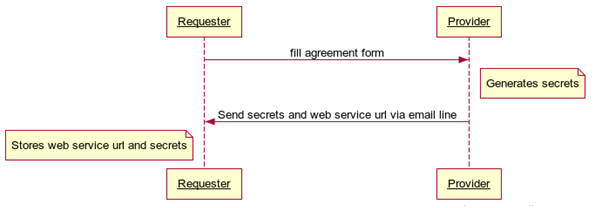
\includegraphics[width=14cm]{sq_agreement.png}
  \caption{Making Exchange Agreement}
  \label{fig:sq_agreement}
\end{figure}


After the implementation of web-service by the provider. The requester fills a form and asks for the credentials. The emails the access point and exchange secrets to the Coordinator.

    \subsection{Find Student Data}
    To find a student record, the requester asks a provider from the agreed providers list for a student record. The provider sends back list of documents associated with the student.

\begin{figure}[!hbp]
  \centering
  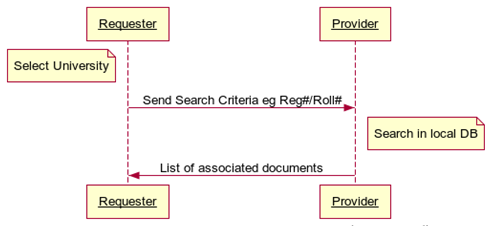
\includegraphics[width=14cm]{sq_find_student_data.png}
  \caption{Finding Student Data}
  \label{fig:sq_find_student_data}
\end{figure}

    \subsection{Exchange a Document Details}
    To exchange a document details, the requester asks a provider with search criteria and document type. The provider sends back the document details using DRESS.

\begin{figure}[!htp]
  \centering
  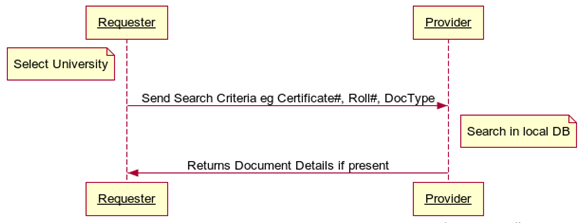
\includegraphics[width=14cm]{sq_exchange_doc.png}
  \caption{Exchanging a Document Details}
  \label{fig:sq_exchange_doc}
\end{figure}

\section{Mapping and Web Service Challange}

It is very important to understand that to implement the scenarios mentioned in section \ref{s-business_process}, every provider must implement a web-service based on DRESS. This is a challenging task since every partaking institute (provider) has different schemas and different database management systems. This schema is required to be mapped to DRESS. This must be served to the requester using a web-service. This creates an opportunity for a semi-automated tool which maps the schemas to DRESS and generate a web-service automatically.

\section{Software Specifications}
Based on the business process and the challenges we discussed, functional and non-functional requirements are;

    \subsection{Functional Requirements}


    \subsection{Non-functional Requirements}


\chapter{Architecture \& Design}\label{ch-architecture-design}
From the requirements analysis, we suggest student exchange system should have distributed architecture. As partaking institutes are autonomous and themselves maintain the its own data. It signs agreements independently for exchanging data with other universities. Each can be a requester plus a provider of data. The circles/nodes in the figure below represent universities. The arrows represent exchange of data.

\begin{figure}[!htp]
  \centering
  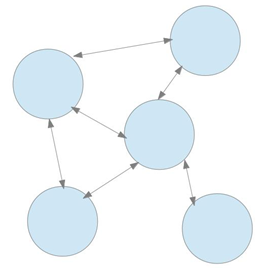
\includegraphics[width=6cm]{architecture_distributed_independent_exchange.png}
  \caption{Multiple Nodes Exchanging Information Independently in Distributed Architecture \cite{The Mobility Project}}
  \label{fig:architecture_distributed_independent_exchange}
\end{figure}

This peer to peer like distribute architecture has benefits over adding a middle agent or central server in the system.

\begin{enumerate}
\item Avoidance from single point of failure.
\item Lesser load.
\item Each university having control over its own data and thus building trust in the system.	
\end{enumerate}

We suggest student exchange system will have distributed architecture. Each university has its own data and signs agreements with HEC for exchanging data with other universities. Each can be a requester plus a provider of data. The circles/nodes in the figure below represent universities

\begin{figure}[!htp]
  \centering
  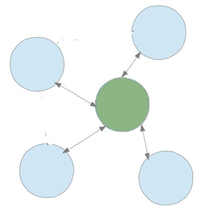
\includegraphics[width=5cm]{architecture_distributed_exchange_through_hec.png}
  \caption{Multiple Nodes Exchanging Information Through a Central Control Authority in Distributed Architecture}
  \label{fig:architecture_distributed_exchange_through_hec}
\end{figure}

There are some choices to be made at this point. We will be using web services for exchanging data as they provide a high abstraction from network issues and use well known standards like XML over HTTP. There are some XML based data exchange protocols on web. These are XML-RPC, SOAP, and REST.

The nodes will exchange data using SOAP based web service in our system.  We chose SOAP as it forces to follow a formal standard and supports developer defined data types.

The number of universities can increase when agreements are signed with new universities for exchange data. The web service URLs need to be saved so that requester can retrieve this URL and request that university. This can be achieved by developing a custom system "URL registry" for saving web services URLs. Now we have to make a choice. URL registry can be global or each requesting node can have its own private URL registry. We will use private registry to avoid single point of failure and to minimize load.

\begin{figure}[!htp]
  \centering
  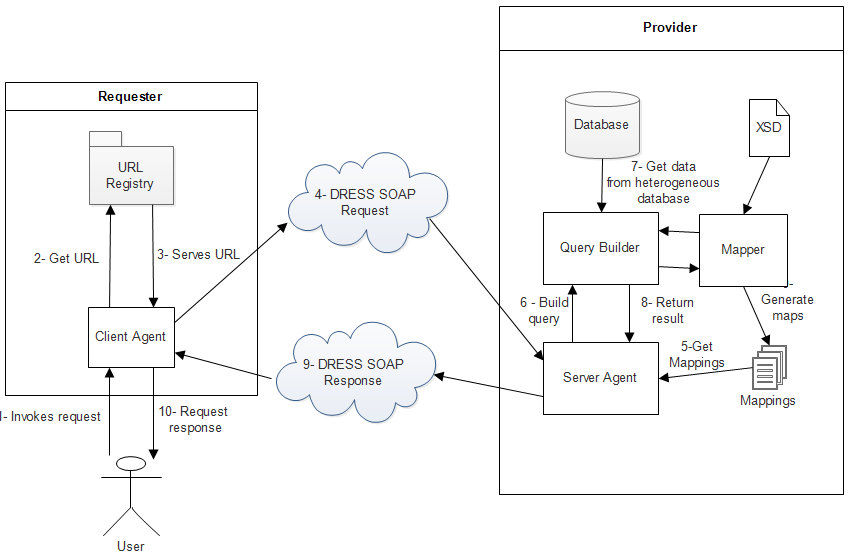
\includegraphics[width=12cm]{architecture.png}
  \caption{Architecture Diagram}
  \label{fig:architecture}
\end{figure}

%%%%%%%%%%%%%%%%%%%%%%%%%%%%%%%%%%%%%%%%%%%%%%%%%%%%%%%%%%%

\chapter{Implementation}\label{ch-implement}
In this chapter, the methodology that is used for modeling is explained.


\chapter{Conclusions}
\label{ch:Conclusions}

\section{This is the End}
\label{sec:This_is_the_end}
%
In this research we reported the design and implementation of.


%\backmatter


\begin{thebibliography}{10}

\bibitem{umair}
M. Ali, H. Qureshi, and M. S. Akhtar (2013), \emph{Analysis of growth in Students Intake and Degree Awarding Contribution: A Comparison of Stanford and MIT}, MLDM 2013: International Conference on Machine Learning and Data Mining, in press.

\bibitem{bologna process}
http://www.ehea.info/Uploads/Irina/Bologna%20beyond%202010.pdf

\bibitem{MAPQFTOOL}
P. Pouyioutas, H. Gjermundrod, and M. Michael, "MAPQFTOOL: A software tool to support national qualifications frameworks," Information Society (i-Society), 2011 International Conference on, pp. 198-203, Jun. 2011.

\bibitem{The Mobility Project}
Rafal Nagrodzki, "The Mobility Project," Institue of Informatics, University of Warsaw, Warsaw, Master's Thesis 2009.

\bibitem{European Higher Education Area }
A. Duran, Y.B. Moon, and E. Giraldo, "Work in progress - the European Higher Education Area ("Bologna process") in Engineering Education in Spain," Frontiers in Education Conference, 2009. FIE '09. 39th IEEE, pp. 1,2, Oct. 2009.

\bibitem{Integration of Services in the Mobility Project}
Karol Kanski, "Integration of Services in the Mobility Project," Institute of Informatics, University of Warsaw, Warsaw, Master's Thesis 2011.

\bibitem{Data integration: the teenage years}
Alon Halevy, Anand Rajaraman, and Joann Ordille, "Data integration: the teenage years," In Proceedings of the 32nd international conference on Very large data bases (VLDB '06), pp. 9-16, 2006.

\bibitem{improvement bologna process}
Szentirmai, L.; Radacs, L., "Improvement of academic and research standards of higher engineering education in light of Bologna process," Emerging eLearning Technologies \& Applications (ICETA), 2012 IEEE 10th International Conference on , vol., no., pp.381,386, 8-9 Nov. 2012

\bibitem{SCHAC 1.5.0}
https://wiki.refeds.org/download/attachments/1606048/SCHAC
\%2B1.5.0.pdf?version=3\&modificationDate=1429195142624\&api=v2

\end{thebibliography}

\end{document} 